\documentclass[12pt]{article}
%\linespread{1}
\usepackage[margin=1.0in]{geometry}

\usepackage{amsmath}
\usepackage{amssymb}
\usepackage{multicol}
\usepackage{graphicx}

\title{Distributed Sampled Convex Problems}
\author{David Eckman (dje88) and Calvin Wylie (cjw278)}
\date{}

\begin{document}

%\noindent
\setlength{\parindent}{24pt}

\maketitle

\section*{Abstract}
It is well-known that chance constrained programs are in general intractable because of the non-convexity of the feasible region and the requirement of prior information about the distribution of the uncertain parameters.
Solving a sampled convex program allows for finding solutions that are feasible for the chance constrained program with high probability with known bounds on the required number of samples.
Sampled convex problems are more easily solved because they are characterized by a finite number of constraints and require only that one can obtain i.i.d. samples of the uncertain parameters.
However, the required number of samples may still result in a sampled convex program that is expensive to solve exactly.
We consider obtaining approximate solutions to these sampled convex programs by distributing the constraints across processors and solving smaller subproblems followed by a consensus on the active constraints.
We consider a classical portfolio-optimization problem and study the trade-offs that arise from this method: including wall-clock time, violation probability, and feasibility probability.

\section*{Introduction}
Chance constrained problems model many real-word applications in areas as diverse as finance, energy, and emergency services \cite{bental09}.
For example, chance constraints can represent an acceptable level of risk in an investment or a fixed level of service that is guaranteed.
A typical chance-constrained program \ref{ccp} is given by
\begin{align}\label{ccp}
\begin{split}
\begin{aligned}
    & \underset{x \in \mathcal{X}}{\text{minimize}}
    & & c^T x \\
    & \text{subject to}
    & & \mathbb{P}\{f(x,\delta) \leq 0\} \geq 1-\epsilon.
\end{aligned}
\end{split} \tag{CCP$_\epsilon$}
\end{align}
where $\mathcal{X} \subseteq \mathbb{R}^n$ is compact, $\delta$ is the uncertain parameter drawn from the uncertainty set $\Delta \subseteq \mathbb{R}^d$ according to a probability measure $\mathbb{P}$, and $f:\mathcal{X} \times \Delta \mapsto \mathbb{R}$ is convex in $x$ for any fixed $\delta$.
The parameter $0 \leq \epsilon \leq 1$ represents the acceptable probability with which the constraint $f(x,\delta) \leq 0$ can be violated.
The problem \ref{ccp} is notoriously intractable for two reasons: (1) that the feasible region is, in general, non-convex, and (2) the distribution $\mathbb{P}$ must be known a priori.

One method for finding solutions with good performance which are also feasible for \ref{ccp} with high probability is to take $N$ iid samples $(\delta_1, \ldots, \delta_N)$ from the uncertainty set $\Delta$ according to $\mathbb{P}$ and solve the corresponding sampled convex program \ref{scp}:
\begin{align}\label{scp}
\begin{split}
\begin{aligned}
    & \underset{x \in \mathcal{X}}{\text{minimize}}
    & & c^T x \\
    & \text{subject to}
    & & f(x,\delta_i) \leq 0 \quad i = 1, \ldots, N.
\end{aligned}
\end{split} \tag{SCP$_N$}
\end{align}
Notice that \ref{scp} is more tractable than \ref{ccp} since it has a finite number of constraints, a convex feasible region, and we need not explicitly know $\mathbb{P}$ but instead only need to be able to obtain iid samples from it.

Let $x_N^*$ be the random solution to \ref{scp} obtained by taking $N$ samples and let $V(x_N^*) = \mathbb{P}^N\{f(x_N^*, \delta) > 0\}$ be the corresponding violation probability where $\mathbb{P}^N$ refers to the product probability measure.
To clarify, if $V(x_N^*) \leq \epsilon$, then $x_N^*$ is feasible for \ref{ccp}, otherwise it is infeasible.

Sampled convex programs do not provide a guarantee that $V(x_N^*) \leq \epsilon$ for a given sample size $N$.
Instead, Calafiore and Campi \cite{campi05} proved that one can bound the number of samples needed to ensure that $\mathbb{P}^N\{V(x_N^*) > \epsilon\} \leq \beta$.
That is, the optimal solution to \ref{scp} is feasible for \ref{ccp} with probability greater than $1 - \beta$.
Their bound of $N \geq 1/(\epsilon\beta) - 1$ is simple to calculate, but is quite loose in terms of asymptotics.
The bound was further tightened to choosing $N$ to satisfy
\[ \mathbb{P}^N\{V(x_N^*) > \epsilon\} \leq \binom{N}{d}(1-\epsilon)^{N-d}. \]
in \cite{campi06} and then later by Campi and Garatti in \cite{campi08} to the solution to a binomial equation:
\[ \mathbb{P}^N\{V(x_N^*) > \epsilon\} = \sum_{i=0}^{d-1} \binom{N}{i} \epsilon^i (1-\epsilon)^{N-i}. \]
Note that all of these bounds are distribution-free which means that $N$ can be calculated without prior knowledge of $\mathbb{P}$.

For modest $\epsilon$ and $\beta$, the required $N$ may be large enough to cause the resulting \ref{scp} instance to be computationally expensive to solve exactly.
Even for instances in which $N$ is modest, but the number of decision variables, $n$, is large, solving \ref{scp} may pose challenges.
When either the decision variables or constraints number in the thousands, existing software for solving mixed integer programs or semi-definite programs might take too long to run to completion.
Without loss of generality, we will assume that the number of constraints is the limiting factor in solving \ref{scp} directly; if the number of decision variables is the issue, one can consider taking the dual of \ref{scp}.

One idea for addressing this challenge is to decompose \ref{scp} into smaller sampled convex programs and solve them in parallel before forming some consensus across the subproblems.
Because the subproblems have only a fraction of the constraints of \ref{scp}, they can be solved faster.
However because each subproblem is only considering a subset of the constraints, there is a loss associated with this simplification: namely the solution returned will likely violate some of the constraints of \ref{scp} and therefore is less likely to be feasible for \ref{ccp}.
Furthermore, because the solution violates some of the constraints, its corresponding objective function value will be less than $c^T x_N^*$ (in the case where the objective is to minimize $c^T x$).
Still, the speedup in terms of wall-clock time due to parallelism may be worth the loss in the probability that the solution is \ref{ccp}-feasible.
%In particular, we would like to study how much is lost with respect to \ref{ccp} feasibility by taking the active constraints from the subproblems and solving a final sampled convex program with these constraints.

\section*{Method}
A feasible convex program in $n$ dimensional space will have at most $n$ support constraints at the optimal solution.
Therefore the problem of finding an optimal solution to \ref{scp} can be viewed as the problem of identifying the $n$ supporting constraints at $x_N^*$.

A recent paper by Carlone et al. \cite{carlone2014} studies solving large-scale convex programs in a distributed fashion.
It assumes a directed graph topology on the communication network connecting the parallel processors.
Initially, each processor is given a subset of the constraints of the master problem with which it solves a convex subproblem.
It then identifies the support constraints at that solution and passes them to other processors according to the network topology.
Each processor receives the incoming constraints and resolves a convex subproblem with their original set of constraints the new constraints.
It was proven that after an almost surely finite number of iterations, all processors will reach a consensus about which constraints are supporting for the solution to the master problem.
Note that the objective in \cite{carlone2014} is to recover the exact solution to the convex program whereas we are interested in finding an approximate solution in less time.

In practice, this procedure would take far too long to run to completion, especially since there is no bound on the number of iterations needed for consensus.
%The only instance you would fully run a procedure like this is if the master problem is too large to solve with existing software.
Instead, we will consider a variation of this procedure which only runs for two iterations and the topology of the communication network is a star graph in which all worker processors pass supporting constraints to a master processor.
Because there are only two iterations, the solutions returned will likely not be the exact solution to \ref{scp}.
However this approximate solution may be calculated in less time, and thus it may be worth a loss in the probability of being a \ref{ccp}-feasible solution.

Suppose that we have available one ``master'' processor and $p$ ``worker'' processors available.
For simplicity, suppose that $N = mp$ for some positve integers $m > n$.

We describe our procedure as follows:

\textbf{Parallel \ref{scp} Procedure}
\begin{enumerate}
\item For each processor $1 \leq j \leq p$, solve the sampled convex program
\begin{equation*}
\begin{aligned}
    & \underset{x \in \mathcal{X}}{\text{minimize}}
    & & c^T x \\
    & \text{subject to}
    & & f(x,\delta_i) \leq 0 \quad i = m(j-1) + 1, \ldots, mj.
\end{aligned}
\end{equation*}
Let $\tilde{x}_j$ be the corresponding solution.
\item For each slave processor $1 \leq j \leq p$, determine the supporting constraints of the 
optimal solution $\tilde{x}_j$.
Assuming that each sampled convex program is fully-supported with probability one,
label the sample corresponding to these constraints $\delta_1^j, \ldots, \delta_n^j$.
Send these samples to the master processor.
\item On the master processor, solve the sampled convex program
\begin{equation*}
\begin{aligned}
    & \underset{x \in \mathcal{X}}{\text{minimize}}
    & & c^T x \\
    & \text{subject to}
    & & f(x,\delta_i^j) \leq 0 \quad i = 1,\ldots,k \text{ and } j = 1,\ldots,p.
\end{aligned}
\end{equation*}
Let $\tilde{x}$ be the corresponding solution.
\end{enumerate}

For each subproblem, we identify the support constraints (of which there should be $n$ unless the problem is degenerate) by checking which constraints are active at $\tilde{x}_j$, i.e. which $\delta_i$ satisfy $f(\tilde{x}_j, \delta_i) = 0$.


Changing the number of processors $p$ has interesting effects on the main performance measures: wall-clock time and $\mathbb{P}\{V(\tilde{x}) > \epsilon\}$.
With more processors, the subproblems are smaller, but the total number of constraints passed to the master program ($np$) is larger.
This will impact the wall-clock time of the procedure in two conflicting ways.
And as the number of constraints in the master problem increases, we would expect $\mathbb{P}\{V(\tilde{x}) > \epsilon\}$ to decrease.
The main research question of this study will be: given these trade-offs, what is the optimal number of processors to use?

Another way to view the problem is to assume with are willing to commit to the wall-clock time need to solve \ref{scp}.
But instead of solving \ref{scp} we want to use the time to take more than $N$ samples and apply the distributed procedure.
Using that time, what is the best number of processors to use and number of constraints to give to each processor and is the performance of the distributed procedure competitive with simply solving \ref{scp}.

Another possible direction to look is to take $\tilde{x}$ as some convex combination of the
optimals solutions from the subproblems.  Intuitively, if each of the subproblems somehow
approximate \ref{ccp}, then somehow ``averaging'' them should give us at least something
no worse.

\section*{Example Problem}

We consider the classical portfolio optimization problem of selecting an allocation of one dollar over $n$ assets with uncertain payouts $r_i$ for $i = 1, \ldots, n$.
Of these assets, we assume that the $n$th asset has a fixed payout (it might, for example, represent a bond with a certain return).
Our objective is to maximize the value-at-risk (VaR) at a risk level of $\epsilon$.
Here VaR is the $\epsilon$-percentile of the distribution of returns for a particular allocation.
Therefore we have the following chance constrained program:
\begin{align}\label{Portfolioccp}
\begin{split}
\begin{aligned}
    & \underset{y, t}{\text{maximize}}
    & & t \\
    & \text{subject to}
    & & \mathbb{P}\left\{ \sum_{i=1}^{n-1} r_i y_i + r_n y_n \geq t \right\} \geq 1-\epsilon \\
    & & & \sum_{i=1}^n y_i = 1 \\
    & & & y_i \geq 0 \quad \forall i = 1, \ldots, n.
\end{aligned}
\end{split} \tag{Portfolio CCP}
\end{align}

Here the chance constrained program models the acceptable level of risk in an investment.
We will assume that the vector of payouts $y$ is distributed according to a multivariate log-normal distribution with mean vector $\mu$ and covariance matrix $\Sigma$.
A log-normal is typical for asset payouts because it is unimodal with support on the positive real line.
Even with knowledge of the probability distribution of the payouts, the feasible region is non-convex. (Is it really?)


From taking samples $r^{(j)}$ for $j = 1, \ldots, N$, the corresponding sampled convex program is 
\begin{align}\label{Portfolioscp}
\begin{split}
\begin{aligned}
    & \underset{y, t}{\text{maximize}}
    & & t \\
    & \text{subject to}
    & & \sum_{i=1}^{n-1} r_i^{(j)} y_i + r_n^{(j)} y_n \geq t \quad j = 1, \ldots, N \\
    & & & \sum_{i=1}^n y_i = 1 \\
    & & & y_i \geq 0 \quad \forall i = 1, \ldots, n.
\end{aligned}
\end{split} \tag{Portfolio SCP$_N$}
\end{align}


\ref{Portfolioscp} has several nice properties:
\begin{itemize}
\item The objective function and constraints of \ref{Portfolioscp} are linear. Therefore we can use the simplex method to solve the sampled convex subproblems.
\item Because of the fixed asset $n$, it is possible to easily find a basic feasible solution by taking $y_n = 1$, $y_i = 0$ for $i = 1, \ldots, n-1$ and $t = r_n$.
\item The feasible allocations $y$ sit within a simplex.
\item Is $t$ also bounded by the some of the VaR for each asset.
\end{itemize}

Here we take $\epsilon = 0.05$ and $\beta = 1 \times 10^{-5}$ to get a required sample size of $N = 5312$.

\section*{Implementation in MPI}

We use MPI for communication across processors and glpk as our simplex solver.


Figure \ref{fig:fig_simplex_time} shows some experimental timings for the simplex and dual simplex methods applied to our problem with $n = 200$.
It shows a superlinear increase in wall clock time with respect to the number of constraints.
This trend is promising for us to decompose the \ref{Portfolioscp} into smaller subproblems to achieve time savings through parallelism.

\begin{figure}[ht]
	\centering
		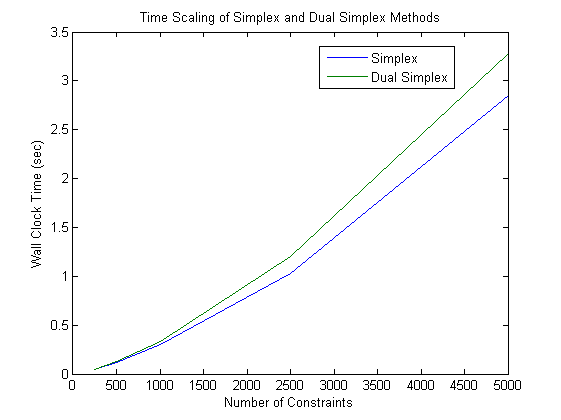
\includegraphics{../plot/figs/fig_simplex_time.png}
	\caption{Wall-Clock Times for Simplex and Dual Simplex}
	\label{fig:fig_simplex_time}
\end{figure}


\section*{Experiments}

However, $V(x_N^*)$ cannot be explicitly calculated unless we have an analytical form for $\mathbb{P}$.
Instead we often resort to estimating $V(x_N^*)$ via Monte Carlo simulation: obtaining $R$ i.i.d. samples of $\delta$ and calculating
\[ \hat{V}(x_N^*) = \frac{1}{R} \sum_{i = 1}^R \mathbf{1}\{f(x_N^*, \delta_i) > 0\}. \]

We take $M$ macro-replications of the procedure and calculate the following point estimates of $E[V(x^{**})]$ and $\mathbb{P}\{V(x^{**}) > \epsilon\}$:
\[ \widehat{E[V(x^{**})]} := \frac{1}{M} \sum_{i=1}^M \hat{V}(x^{**}), \]
and
\[ \widehat{\mathbb{P}\{V(x^{**}) > \epsilon\}} := \frac{1}{M} \sum_{i=1}^M \mathbf{1}\left(\hat{V}(x^{**}) > \epsilon\right). \]
We use exact binomial tests (Clopper-Pearson) to form approximate confidence intervals for these two performance measures.

\begin{figure}[ht]
	\centering
		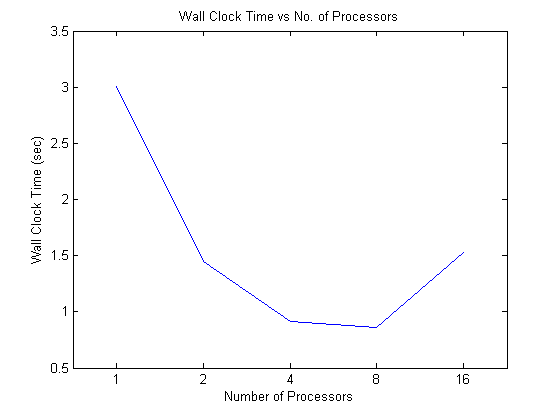
\includegraphics{../plot/figs/wct_numproc.png}
	\caption{Wall-Clock Times by Number of Processors}
	\label{fig:wct_numproc}
\end{figure}

\begin{figure}[ht]
	\centering
		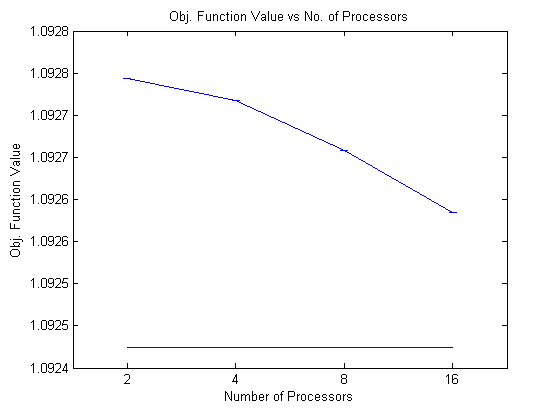
\includegraphics{../plot/figs/objfnval_num_proc.png}
	\caption{VaR $t^*$ by Number of Processors}
	\label{fig:objfnval_num_proc}
\end{figure}

\begin{figure}[ht]
	\centering
		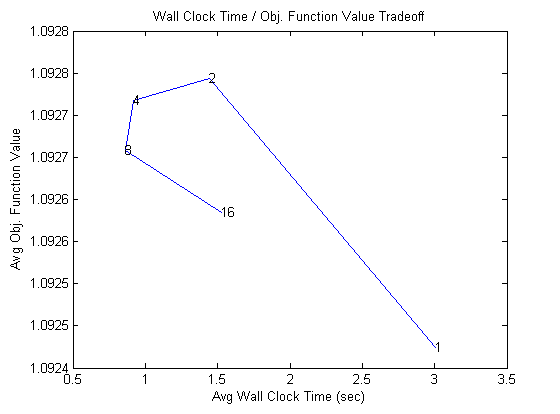
\includegraphics{../plot/figs/wct_objfnval_frontier.png}
	\caption{Trade-off between Time and Var $t^*$}
	\label{fig:wct_objfnval_frontier}
\end{figure}

\begin{figure}[ht]
	\centering
		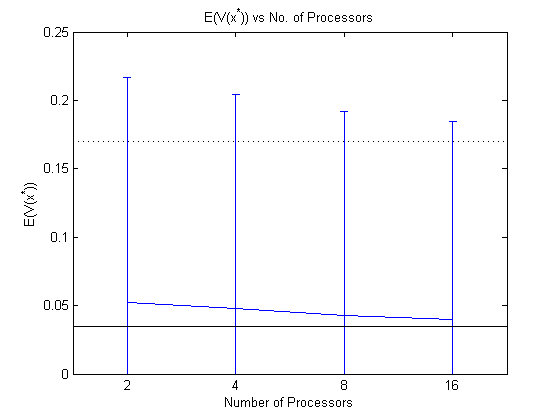
\includegraphics{../plot/figs/expviolprob_numproc.png}
	\caption{$E[V(x^{**})]$ by Number of Processors}
	\label{fig:expviolprob_numproc}
\end{figure}

\begin{figure}[ht]
	\centering
		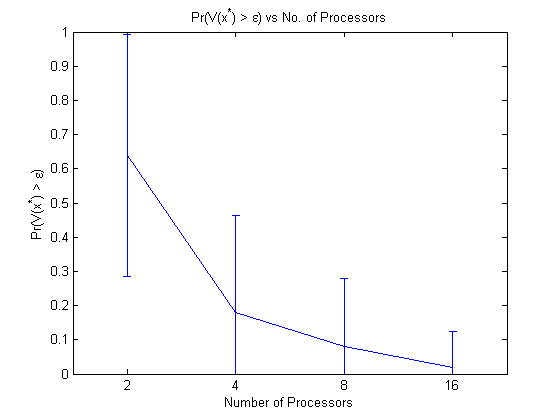
\includegraphics{../plot/figs/probviolprobgreateps_numproc.png}
	\caption{$\mathbb{P}\{V(x^{**}) > \epsilon \}$ by Number of Processors}
	\label{fig:probviolprobgreateps_numproc}
\end{figure}

\begin{figure}[ht]
	\centering
		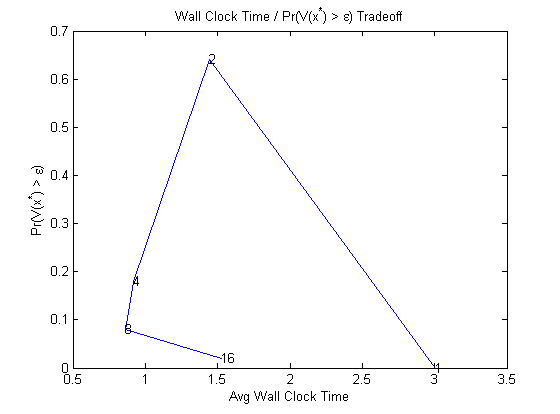
\includegraphics{../plot/figs/wct_probviolprobgreateps_frontier.png}
	\caption{Trade-off between Time and $\mathbb{P}\{V(x^{**}) > \epsilon \}$}
	\label{fig:fig_simplex_time}
\end{figure}


Sensitivity analysis (maybe).
\section*{Performance Analysis}

\section*{Conclusions}



%We intend to conduct experiments on the performance of the parallel procedure versus the traditional serial \ref{scp} procedure.
%For measures of performance of the solutions $x^*$ and $x^{**}$, we will look at the objective function values, the expected violation probabilities, and the probabilities that the violations probabilities are greater than $\epsilon$.
%We will make comparisons based on both the total number of samples and the total wall-clock times of the two procedures.
%
%We will also experiment with variations of the basic procedure.
%One variation would involve communicating the support constraints of the master's problem back to the slaves and doing new sampling before solving new subproblems for each slaves.
%This could be done over a number of iterations and we could study the performance of the returned solutions at each iteration.
%
%Another variation would again involve communicating support constraints of the master's problem back to the slaves, but instead of doing new sampling, we re-solve the subproblems with the additional shared support constraints.
%After sending the support constraints of these new subproblems to the master, we could perform one final solve and get a solution that is no worse than the previous.
%This is because passing support constraints from the master to the slaves would allow for constraints that were not previously support constraints to become support constraints.

\bibliographystyle{siam}
\bibliography{references} 

\end{document}